\chapter{Estrategia Empírica}

\noindent En este capítulo, analizo el impacto que tuvieron las cámaras de velocidad del programa de fotocívicas sobre la seguridad vial en la Ciudad de México. En particular, estudio cómo la instalación de estos radares afecta el número y la severidad de los incidentes viales, poniendo especial énfasis en los accidentes con lesionados y con víctimas fatales. A partir de la literatura revisada, planteo la hipótesis de que las cámaras generan una reducción de estos incidentes en el entorno inmediato donde operan, aproximadamente en un radio de 300 metros alrededor de cada dispositivo.\\

Para poner a prueba esta hipótesis, construyo distintas áreas de influencia en torno a las cámaras y estimo su efecto con un solo diseño que combina dos herramientas, con información de incidentes viales proveniente del C5: el \textit{propensity score matching} selecciona zonas sin cámara comparables a las áreas tratadas, y un modelo de diferencias en diferencias compara la evolución de los incidentes en ambos grupos antes y después del programa. En las secciones que siguen, primero presento el marco conceptual que motiva mis hipótesis y los mecanismos a través de los cuales los radares de velocidad podrían modificar la ocurrencia y gravedad de los accidentes. Después, explico cómo, a partir de este marco conceptual y de las características de los datos disponibles, llego a la estrategia de identificación final. Finalmente, hago explícitos los supuestos bajo los cuales mis resultados pueden interpretarse de manera causal y discuto el alcance y las limitaciones de esta interpretación.\\

\section{Marco Conceptual}
\subsection{Velocidad y dinámica del flujo vehicular}
\noindent Una de las vías más directas a través de las cuales las cámaras de velocidad pueden afectar la seguridad vial es modificando la velocidad a la que circulan los vehículos y, con ello, la dinámica del flujo vehicular en su entorno. A mayor velocidad aumenta tanto la probabilidad de que ocurra un siniestro como la severidad del mismo, dado que el conductor tiene menos tiempo y distancia para reaccionar (García, 2018).\\

\indent Las cámaras de velocidad actúan precisamente sobre ese canal: generan un incentivo a reducir la velocidad, al aumentar la probabilidad percibida de sanción en un punto específico de la vialidad. Sin embargo, este efecto rara vez corresponde a una reducción uniforme de la velocidad a lo largo de un tramo completo, sino que más bien se traduce en lo que se conoce como el efecto ``canguro'': una disminución abrupta antes del radar de velocidad y una aceleración una vez que se ha salido del área de efectividad (Li et al., 2013 y 2020; Graham et al., 2019; Mountain et al., 2005; De Pauw et al., 2014).\\

En un contexto urbano como la Ciudad de México, es razonable anticipar dinámicas similares, que pueden tener impactos distintos en el número de incidentes. Por un lado, la reducción de velocidad en el área de influencia puede disminuir los accidentes y su severidad al darle más tiempo de reacción y de frenado al conductor, y disminuyendo la severidad en caso de presentarse un incidente. Por otro lado, la forma en la que los conductores ajustan su comportamiento no es homogénea: no solo existe diferencia entre aquellos que respetan de manera estricta el límite de velocidad y aquellos que solo lo hacen cuando su riesgo de ser detectados es más alto, sino que recordemos que las sanciones en Ciudad de México tampoco son iguales para todos los conductores, y están sujetas a la placa de registro del vehículo. Esta heterogeneidad de respuestas genera cambios no solo en el nivel medio de velocidad, sino también en su variabilidad.\\

En vías donde coexisten vehículos muy lentos con otros muy rápidos tienden a registrar mayores tasas de incidentes que vías donde todos los vehículos circulan a una velocidad similar (Aart, Schagen, 2005; Choudharya et al., 2018; Wang et al., 2018). Bajo este argumento, un esquema de control que induce a algunos conductores a frenar de manera brusca y a otros a mantener velocidades altas puede, localmente, aumentar el riesgo de choques por alcance, maniobras evasivas y conflictos entre carriles, aun cuando la velocidad promedio en el tramo se reduzca.\\ 

Por ello, un análisis de los efectos de las cámaras de velocidad debe poner especial atención a los cambios en las inmediaciones más cercanas de los radares y elegir controles que capten las características del entorno vial y del flujo vehicular, de modo que sea posible aislar el efecto específico de la cámara de otros factores que influyen en la ocurrencia y severidad de los incidentes. Al mismo tiempo, debe evitar áreas tan extensas que hagan que el efecto se diluya.\\ 

\subsection{Migración potencial de accidentes y ausencia de datos de flujo vehicular}
\noindent Una segunda vía a través de la cual las cámaras de velocidad pueden afectar el número y la severidad de los incidentes viales es mediante la migración de los accidentes asociada a cambios en las rutas de los conductores. La literatura documenta que es posible que la presencia de radares induzca a algunos usuarios a elegir vías alternativas para evitar el riesgo de sanción (Mountain, 2005; Li et al., 2013). En principio, controlar por el volumen de tráfico en el tramo permitiría distinguir si las variaciones en la siniestralidad se deben a cambios en la exposición al riesgo o a un efecto real de las cámaras. Sin embargo, en contextos donde no es posible acceder a información detallada de flujo vehicular ---como es el caso en la Ciudad de México---, la evaluación de efectos en áreas, en lugar de limitarse al tramo puntual de la cámara, ofrece una forma de mitigar este problema hasta cierto punto (Li et al., 2020; Christie et al., 2003).\\

\indent Cambios en las trayectorias pueden tener varias consecuencias simultáneas. Por un lado, podrían modificar el flujo vehicular tanto en la vía con la cámara como en calles aledañas, liberando parcialmente la primera y concentrando vehículos en las segundas. Por otro lado, la composición vehicular de los conductores en cada ruta también puede alterarse: usuarios más aversos al riesgo o más sensibles a las multas podrían evitar de forma sistemática los corredores con radares de velocidad, mientras que conductores menos aversos seguirían transitando por esas vías.\\

En ausencia de datos de flujo vehicular que permitan estudiar variaciones en las inmediaciones de los radares de velocidad, es necesario encontrar una forma de capturar estas posibles redistribuciones de tráfico, ya que de no hacerlo, podría confundirse una simple reasignación espacial de los accidentes con una reducción genuina del riesgo. Evaluar el impacto de las cámaras a nivel de áreas de influencia que incluyan tanto el entorno inmediato del radar como sus proximidades ayuda a incorporar, al menos parcialmente, los siniestros que pudieran estar desplazándose hacia calles cercanas.\\

\subsection{Ventana temporal de análisis}
\label{sec:ventana}
\noindent Para determinar el horizonte temporal de análisis es necesario equilibrar tres consideraciones: capturar con suficiente detalle la dinámica previa a la intervención; observar la evolución de sus efectos una vez implementada; y limitar el horizonte para que los periodos que se comparan sigan siendo razonablemente homogéneos entre sí. La literatura sobre cámaras de velocidad se mueve justamente dentro de ese equilibrio. Por un lado, evita tratarlas como intervenciones de efecto permanente e inmutable; en su lugar, define ventanas de tiempo finitas y comparables. Li et al. (2013) fijan un periodo 1999–2007 que, para cada sitio, garantiza tres años de información antes y tres después de la instalación, y dentro de ese marco analizan distintas bandas espaciales. En un trabajo posterior, Li et al. (2020) mantienen la idea de un bloque pretratamiento de tres años, pero prestan especial atención a la evolución del efecto: dividen los doce años posteriores en ventanas de igual longitud, precisamente para no mezclar en una sola estimación periodos que pueden tener comportamientos distintos, y efectivamente encuentran que el impacto se va diluyendo con el paso del tiempo. Christie et al. (2003) siguen una lógica similar al trabajar con una serie 1996–2000 y definir periodos before–after de varios años para estabilizar las tasas locales de choques en cada banda.\\

La comparación sistemática que hacen Li et al. (2013) de distintos estudios muestra que la elección del horizonte responde a objetivos analíticos distintos, más que a una regla única sobre qué ventana es correcta. Horizontes muy largos ---de hasta diez años de choques como Hess y Polak (2003) o Newstead y Cameron (2003)--- son útiles cuando se busca modelar con detalle tendencias de fondo. En el otro extremo, trabajos con ventanas muy cortas, del orden de un año y medio en total, como Shin et al. (2009), son adecuados para capturar cambios casi inmediatos tras la instalación de los radares, aun a costa de una mayor variabilidad por fluctuaciones viales. Entre estos dos extremos, los estudios que intentan evaluar efectos locales y relativamente estables en el tiempo tienden a converger en esquemas de tres años antes y tres años después de la instalación (Mountain et al, 2004, 2005; Gains et al., 2004, 2005; Li et al., 2013). Dado que mi objetivo es precisamente identificar el efecto local de las cámaras, controlando por tendencias generales sin comparar contextos que sean muy distintos entre sí, una ventana simétrica de tres años previos y tres años posteriores resulta la opción más adecuada.\\

La ventana va del 22 de abril de 2016 al 21 de abril de 2022, con la entrada en vigor de las fotocívicas, el 22 de abril de 2019, como punto de corte. Los periodos mensuales se cuentan del día 22 de cada mes al 21 del siguiente, y no por meses de calendario: así, el corte coincide exactamente con el inicio de un periodo, ningún periodo mezcla días anteriores y posteriores al programa, y la ventana queda simétrica, con 36 periodos de cada lado.

Cabe destacar que esta ventana de tres años y tres años después enfrenta un reto crucial: abarca el periodo de la pandemia por Covid-19, que alteró de manera drástica los patrones de movilidad. A partir de marzo de 2020, las restricciones sanitarias y el confinamiento redujeron de forma importante los desplazamientos diarios. De acuerdo con la Secretaría de Movilidad (SEMOVI, 2024), el Sistema de Movilidad Integrada registró una disminución del 45\% en el tránsito vehicular respecto a los niveles previos a la pandemia. Como era de esperarse, esto se tradujo en una caída en el número total de incidentes viales, pero también en un aumento en su severidad, atribuido por la SEMOVI a menores niveles de congestión que facilitaban el tránsito a velocidades más altas. Por ello, si el programa se evaluara solo comparando los incidentes antes y después de su implementación, la caída asociada a la pandemia se confundiría con un efecto de las cámaras.\\

Este problema se aborda de dos maneras. La primera se refiere a la parte del choque que fue común a toda la ciudad: las zonas de control también vivieron la pandemia, por lo que, al comparar la evolución de las áreas tratadas con la de sus controles, esa parte se cancela. Por eso es importante que los controles sean zonas comparables a las tratadas, y no cualquier vialidad de la ciudad. La segunda se refiere a la parte del choque que pudo afectar de forma distinta a las áreas con cámara y a sus controles, por ejemplo si el tránsito cayó más en las vialidades donde se ubican los radares. Esta parte no se corrige, sino que se evalúa, estimando el efecto por separado para cada año del periodo posterior, para verificar que la pandemia no cargue los resultados que se encuentren.\\

Para poder corregir realmente el choque harían falta datos de flujo vehicular en las inmediaciones de cada cámara, que no existen para la Ciudad de México. La única serie de volumen vehicular disponible proviene de los radares de conteo permanente de las casetas de peaje, ubicadas en la periferia de la ciudad: es una sola serie para todas las unidades, no es claro que refleje lo que ocurre en el interior de la ciudad y, al incorporarla al modelo, la absorben por completo los efectos fijos de tiempo. Por ello, las casetas se usan únicamente para describir la magnitud de la caída en la movilidad. Como aproximación a la movilidad local se usa la afluencia mensual promedio de las estaciones del Metro ubicadas dentro de cada área durante los tres años previos al programa, que entra como característica de cada unidad tanto en el emparejamiento como, interactuada con el periodo posterior, en el modelo de diferencias en diferencias.\\

\section{Identificación de supuestos y selección de la muestra}
\subsection{Independencia condicional}
\noindent El emparejamiento por \textit{propensity score} se apoya en el supuesto de independencia condicional: condicionando en un conjunto adecuado de covariables observables, la decisión de instalar una cámara de velocidad en un área dada es “tan buena como aleatoria” con respecto a los resultados de seguridad vial que se analizan (Angrist y Pischke, 2009). En esta tesis, sin embargo, el emparejamiento no es el método de estimación, sino la herramienta con la que se construye un grupo de control comparable; el supuesto que permite interpretar el efecto de manera causal es el de tendencias paralelas, que se discute en la siguiente subsección. Aun así, la independencia condicional ayuda a entender por qué ese grupo de control debe construirse con cuidado.\\

En la práctica, la asignación de cámaras de velocidad dista de ser aleatoria. En particular, durante la implementación del programa de Fotoc\'ivicas, las autoridades reubicaron los radares hacia tramos caracterizados por mayor incidencia de hechos de tránsito, poniendo especial énfasis en aquellos con más personas muertas y lesionadas, así como en puntos con altos volúmenes de tránsito y donde el límite de velocidad se incumplía con mayor frecuencia (SEMOVI, 2019). Es decir, los tramos tratados ya eran, antes de la instalación, sistemáticamente más riesgosos que los no tratados. Una comparación directa entre ambos grupos sin un ajuste cuidadoso heredaría este sesgo de selección y sobreestimaría, o subestimaría, el verdadero efecto de las cámaras.\\

\subsection{Tendencias paralelas}
\noindent La discusión del supuesto de independencia condicional deja claro por qué no es creíble comparar directamente cualquier área con cámara contra cualquier área sin cámara, y por qué es necesario construir un grupo de control comparable a partir de covariables observables. Sin embargo, como la estrategia final de esta tesis no se limita al emparejamiento, sino que combina \emph{propensity score matching} con diferencia en diferencias, hace falta introducir un supuesto adicional de naturaleza temporal: el de tendencias paralelas. En este contexto, dicho supuesto establece que, en ausencia del programa de Fotoc\'ivicas, la diferencia en siniestralidad entre las áreas tratadas y las áreas de control se habría mantenido estable a lo largo del tiempo. Esto no implica que ambos grupos deban partir del mismo nivel de accidentes; lo importante es que, sin intervención, hubieran seguido trayectorias similares. Bajo este supuesto, la evolución del grupo de control puede utilizarse como una aproximación del contrafactual del grupo tratado.\\

Este supuesto es especialmente relevante en este análisis porque el contrafactual de las áreas tratadas no es observable: una vez instaladas las cámaras, ya no es posible ver directamente qué hubiera ocurrido con esas mismas zonas si no hubieran recibido el tratamiento. El \emph{propensity score matching} ayuda a que la comparación sea más creíble al emparejar áreas con características observables similares, pero no sustituye el supuesto temporal que exige la diferencia en diferencias. En otras palabras, el matching mejora la comparabilidad inicial entre grupos, mientras que el supuesto de tendencias paralelas es el que permite usar la trayectoria de los controles emparejados como aproximación de lo que hubiera pasado con las áreas tratadas en ausencia del programa. Por ello, para interpretar de manera causal el coeficiente de interacción entre tratamiento y periodo posterior, es necesario mostrar que las trayectorias previas entre áreas tratadas y controles emparejados son razonablemente comparables.\\

Es aquí donde ambas herramientas se complementan. Entre las covariables del \textit{propensity score} se incluye la tendencia de los incidentes en los tres años previos al programa, de modo que el emparejamiento no solo busca zonas con niveles de siniestralidad similares, sino también con trayectorias previas similares; es decir, el emparejamiento está pensado para hacer más creíble el supuesto de tendencias paralelas. En el capítulo 4 este supuesto se verifica con un \emph{event study} sobre los años previos al programa.\\

\subsection{Restricciones de la muestra y construcción de las áreas de análisis}
\noindent La evaluación del efecto de las cámaras de velocidad exige definir con precisión el universo de estudio y la unidad espacial de análisis. En esta sección describo cómo se restringe la muestra y cómo se construyen las áreas tratadas y de control.\\

\textbf{Unidad de análisis}. Como ya se ha ido adelantando, en este caso la unidad de análisis corresponde a áreas circulares concéntricas en los radares de velocidad, sin embargo, conviene entender el primer enfoque que se tuvo para poder evaluar los beneficios de estas de forma más adecuada. Este primer enfoque consistió en superponer sobre la Ciudad de México una malla regular de celdas cuadradas. Cada celda que contenía al menos una cámara de velocidad se definía como \emph{área tratada}, mientras que las celdas sin cámaras se consideraban como posibles \emph{controles}. Para reducir la heterogeneidad entre celdas, se imponía además que cada celda tuviera traslape con alguna vía primaria de la ciudad.\\

Sin embargo, este enfoque resultó ser muy sensible a decisiones arbitrarias en la construcción de la malla. En particular, pequeñas variaciones en el \emph{offset} del grid (desplazamientos horizontales o verticales en el orden de 10 metros en la posición de origen) cambiaban la distancia entre las cámaras y el centro de sus respectivas celdas, lo que en algunos casos dejaba a la cámara muy cercana al borde de la celda y, por lo tanto, fuera del área donde se esperaría observar su efecto. Como consecuencia, estimaciones que eran estadísticamente significativas con una malla determinada dejaban de serlo con una ligera modificación del grid, aun manteniendo el mismo tamaño de celda. Se exploró una variante en la que se seleccionaba, para cada tamaño de celda, la malla que minimizara la distancia entre cada cámara y el centro de su celda, al tiempo que maximizara la longitud de vías primarias contenidas en cada celda. No obstante, los resultados seguían siendo poco robustos a cambios mínimos en la configuración del grid. Dado que esta falta de robustez cuestiona la credibilidad de las inferencias causales, descarté este enfoque.

Para superar estos problemas, opté por definir áreas de análisis centradas directamente en los puntos donde se ubican las cámaras de velocidad. En concreto, para cada unidad tratada se construyen áreas circulares concéntricas con radios de 100, 150, 200, 250 y 300 metros. Estos radios permiten estudiar cómo varía el efecto de las cámaras conforme se amplía el área alrededor del punto de control, siguiendo la práctica habitual en la literatura que analiza efectos locales de intervenciones puntuales sobre la seguridad vial. Como los círculos están anidados, es decir, el de 300 metros contiene al de 100 metros, cada estimación corresponde al efecto de un área determinada y no a una distancia específica del radar. En la sección de resultados se presentan las estimaciones para cada radio por separado.\\

Con esta redefinición, la distancia al radar deja de depender de cómo se dibuja una malla y pasa a formar parte directa del análisis. Así, en lugar de comparar resultados que cambian por decisiones arbitrarias de partición espacial, es posible observar de manera más clara si el efecto se concentra cerca de la cámara o si se diluye conforme aumenta el radio.\\

\textbf{Cámaras cercanas entre sí}. Algunas cámaras están tan cerca unas de otras que sus círculos prácticamente coinciden. Tratarlas como unidades independientes contaría dos veces la misma zona, por lo que dos cámaras se agrupan en una sola unidad cuando sus círculos de 300 metros comparten más del 60\% de su área. El centro de cada unidad es el promedio de las ubicaciones de sus cámaras. Con esta regla, las 113 cámaras del programa forman 99 unidades tratadas. Los grupos se definen una sola vez, en el radio de 300 metros, y se mantienen en todos los radios. Con esto, el centro de cada unidad queda fijo: los cinco círculos de una misma unidad comparten el mismo centro y el mismo conjunto de cámaras, y lo único que cambia entre estimaciones es el radio. Cuando los círculos de dos unidades distintas se traslapan parcialmente, los incidentes que caen en el área compartida se reparten en partes iguales entre las unidades que la contienen.\\

\textbf{Controles}. La definición de áreas tratadas resuelve el problema de robustez, pero plantea un nuevo reto: es necesario construir un universo de áreas comparables que puedan fungir como controles. Para ello, sorteo 20,000 puntos al azar sobre la red de vías primarias y de acceso controlado de la Ciudad de México, con una probabilidad proporcional a la longitud de cada tramo, de modo que cada metro de vía tiene la misma probabilidad de recibir un punto. Cada punto es el centro de un posible círculo de control. Se descartan los puntos que quedan a menos de 600 metros del centro de alguna unidad tratada, lo que garantiza que ningún control se traslape con un área tratada, incluso en el radio más grande. Quedan 14,656 candidatos, alrededor de 148 por cada unidad tratada, y los mismos centros se usan en los cinco radios. Una vez seleccionados los controles tras el emparejamiento, impongo además una separación mínima de dos radios entre sus centros, de modo que no exista traslape entre ellos y que todos los controles analizados sean también independientes entre sí.\\

Los controles se ubican únicamente sobre vías primarias y de acceso controlado porque son las jerarquías viales donde el programa instaló sus cámaras: un control en una vía donde nunca se habría instalado un radar no aporta un contrafactual creíble.\\ 

Esta decisión se fundamenta, además, en las diferencias estructurales entre vías primarias y secundarias. La red vial de la Ciudad de México tiene una traza anular (Guía para el control de la velocidad, 2018), lo que deriva en vías primarias que concentran el flujo entre el centro y la periferia, operan a mayores velocidades, y dada la definición de traza anular, funcionan como ``barreras urbanas'' que separan barrios y colonias. Las vías secundarias y calles locales, en contraste, actúan principalmente como alimentadoras y desahogo hacia las primarias, con límites de velocidades menores y un entorno predominantemente residencial.\\

El propio marco normativo distingue explícitamente entre tipos de vía. El Artículo 9 del Reglamento de Tránsito de la Ciudad de México establece que, en ausencia de señalamiento específico, los límites generales de velocidad son crecientes con la jerarquía vial: 80 km/h en carriles centrales de vías de acceso controlado (fracción I), 50 km/h en vías primarias (fracción II) y 40 km/h en vías secundarias, incluyendo laterales de vías de acceso controlado (fracción III). En zonas de tránsito calmado el límite desciende a 30 km/h (fracción IV), mientras que en zonas escolares, de hospitales, asilos, la velocidad máxima es de 20 km/h (fracción V). El propio reglamento asume que las vías primarias y de acceso controlado operan a velocidades mayores, lo que sugiere también mayores niveles de exposición al riesgo vial.\\ 

La evidencia descriptiva es coherente con este diagnóstico. Utilizando una agregación espacial en hexágonos de aproximadamente 428 metros de largo (considerando la diagonal mayor), el promedio mensual de accidentes en el periodo previo al tratamiento (2016--2019) es de $2.36$ siniestros (desviación estándar de $1.4$) en hexágonos que contienen alguna vía primaria, frente a $1.33$ siniestros mensuales (desviación estándar de $0.36$) en aquellos que no cuentan con vías primarias (Figura~\ref{fig:accidentes-hexagonos-mapa}). Las distribuciones de accidentes (Figura~\ref{fig:accidentes-hexagonos-dist}) muestran, además, colas más pesadas en las áreas con vías primarias, mientras que las áreas sin ellas se concentran en valores bajos.\\

\begin{figure}
    \centering
    \caption{Promedio mensual de accidentes en la CDMX (2016 - 2019)}
    \label{fig:accidentes-hexagonos-mapa}
    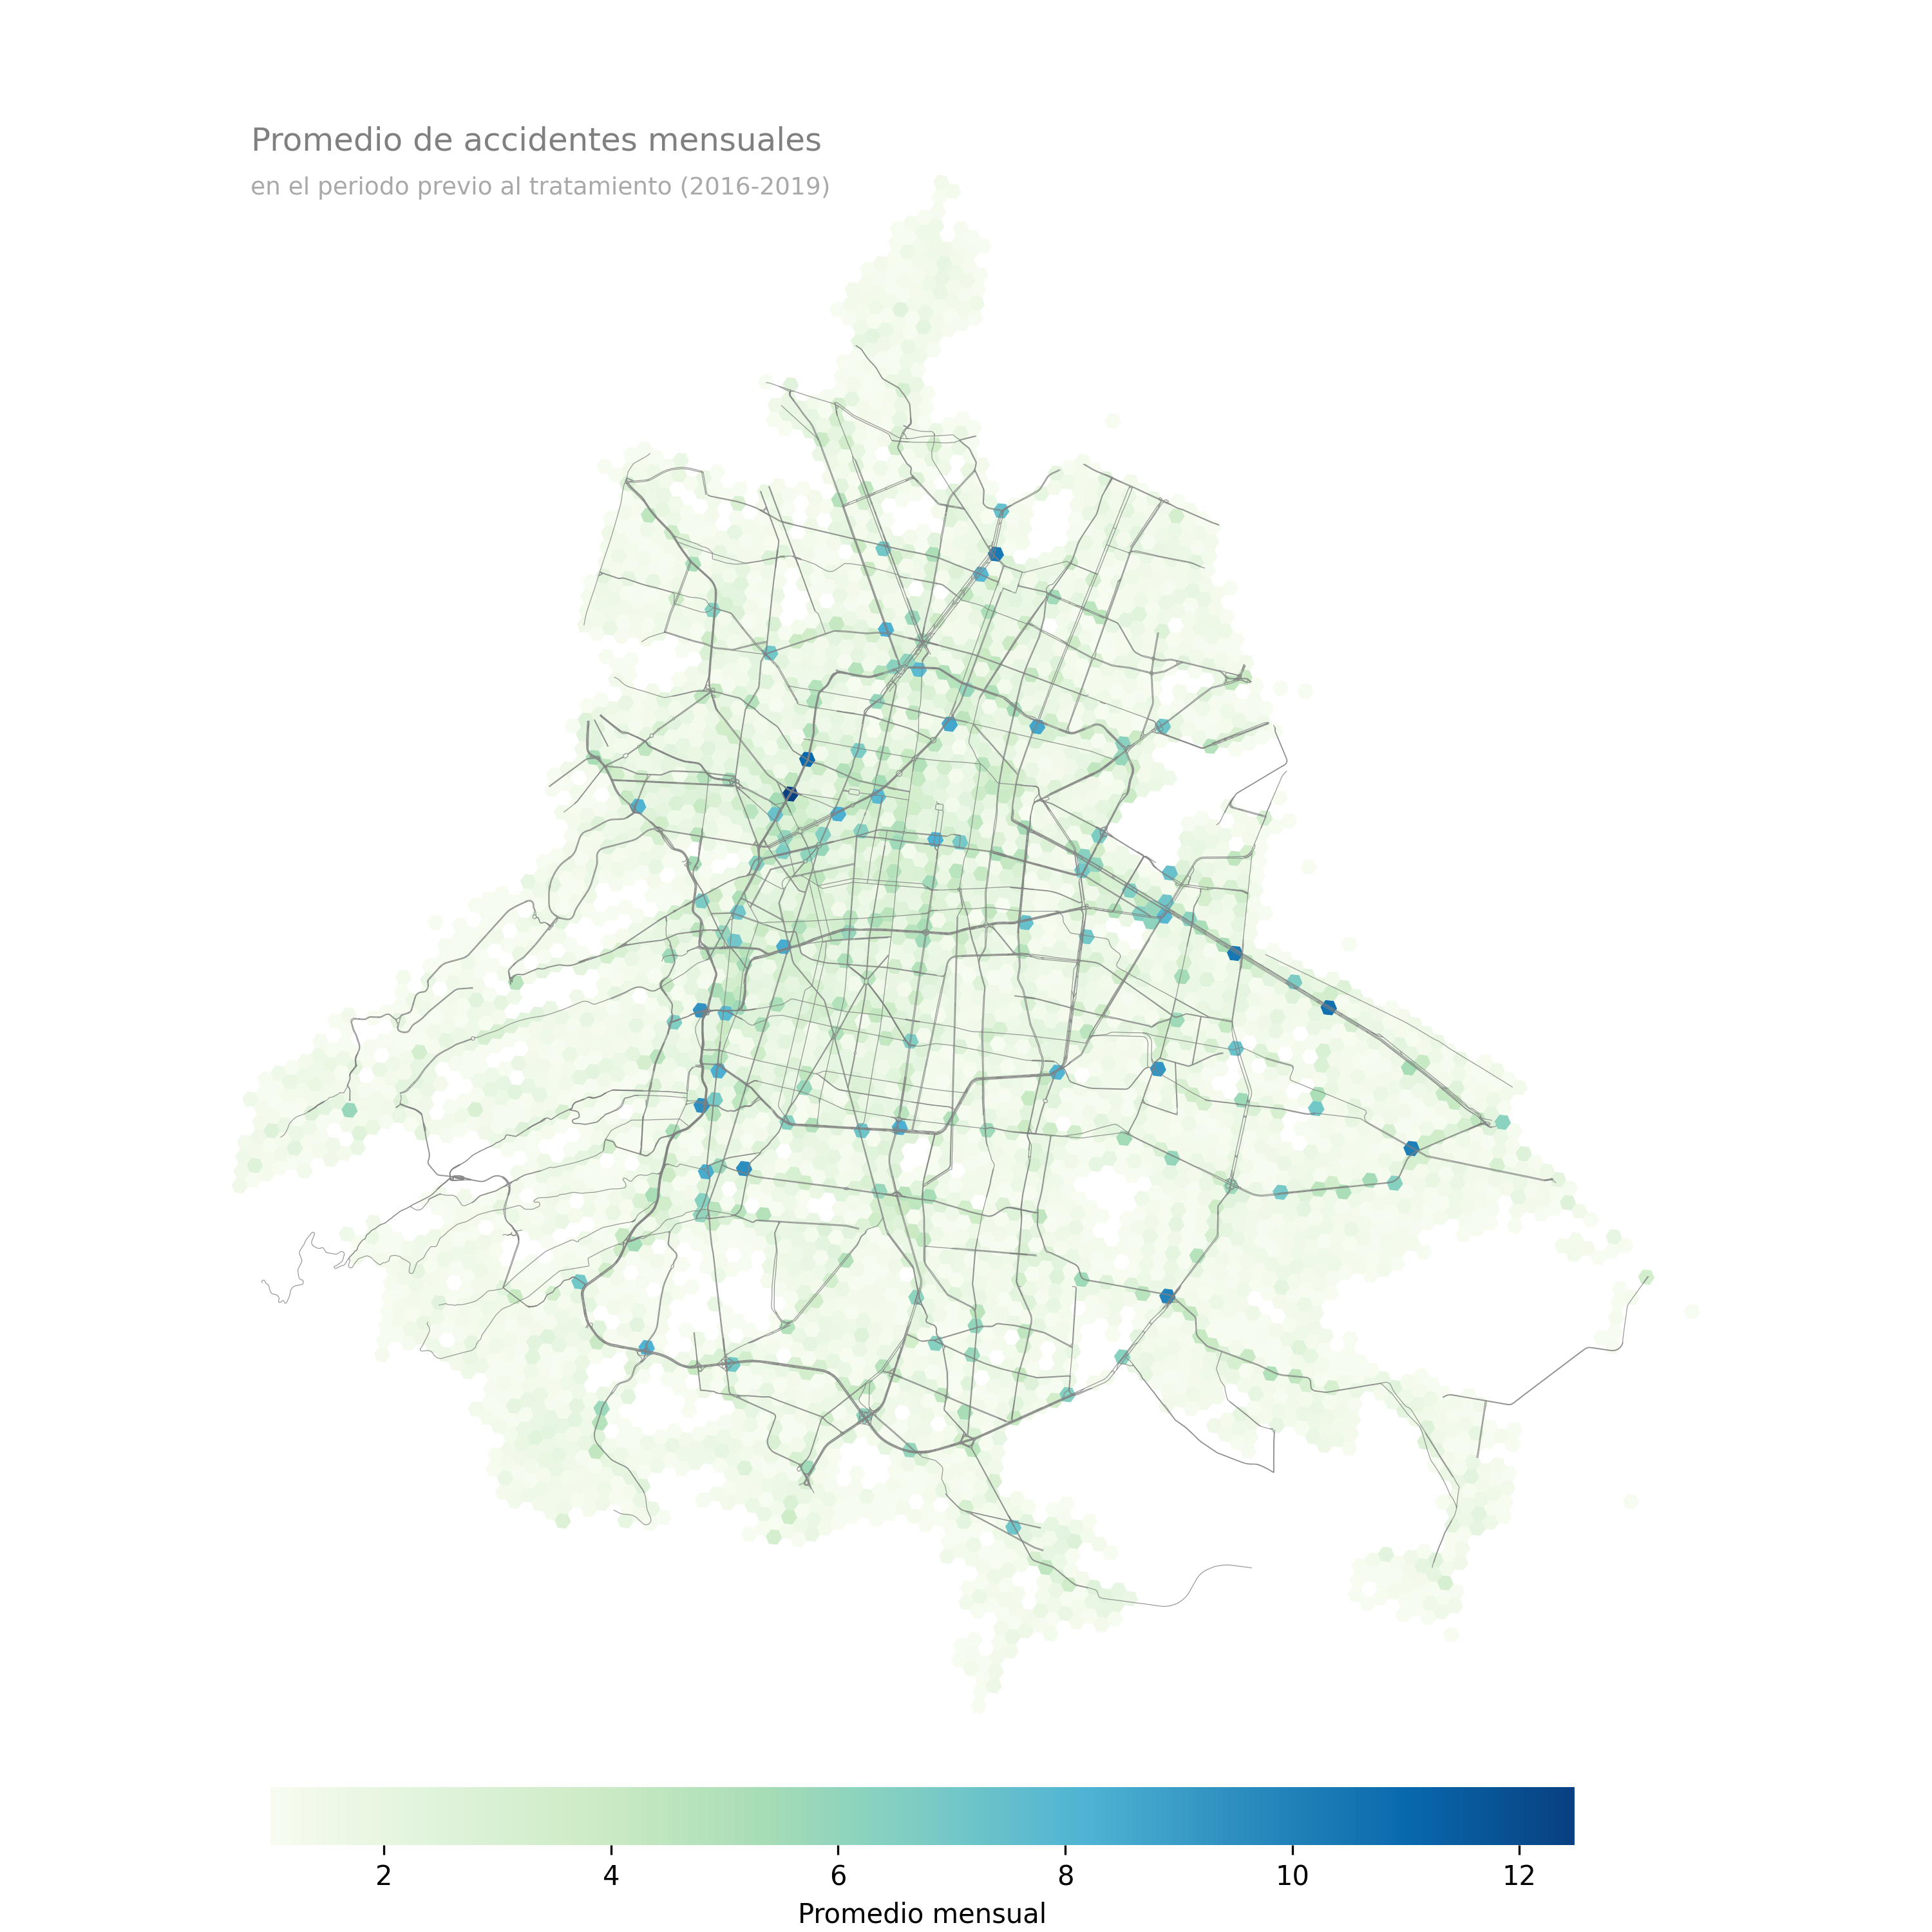
\includegraphics[width=1\linewidth]{Imagenes/promedio-accidenes-mensuales-pre-tratamiento-choroplet.png}
\end{figure}

\begin{figure}
    \centering
    \caption{Distribución de promedio de accidentes mensuales (2016-2019)}
    \label{fig:accidentes-hexagonos-dist}
    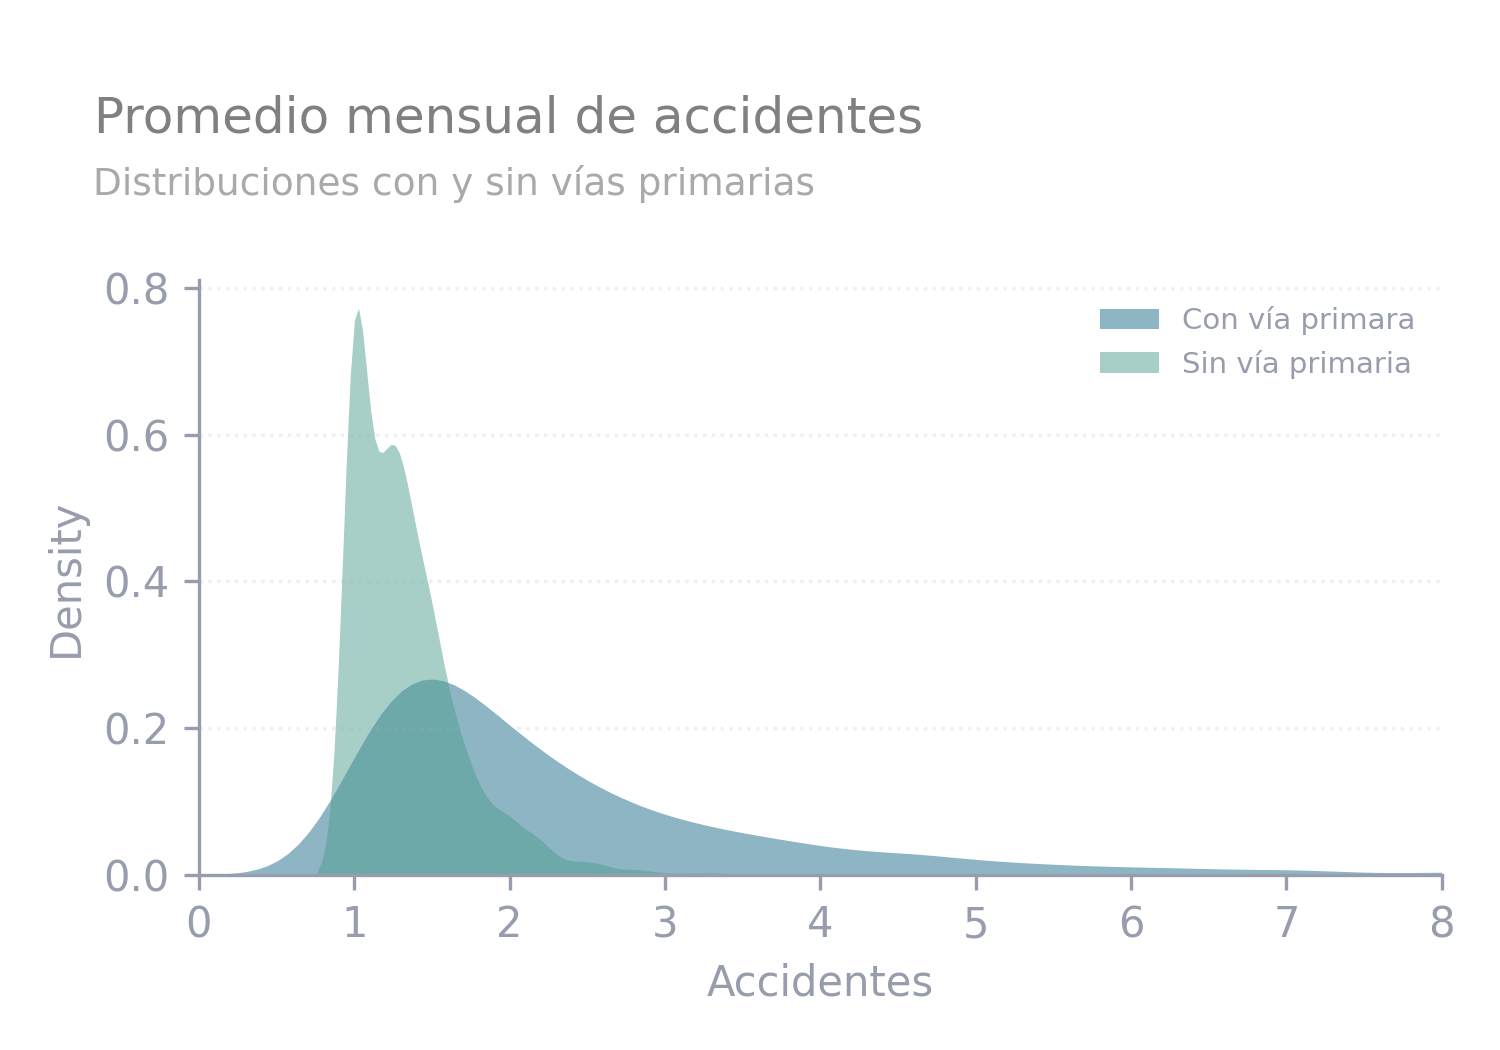
\includegraphics[width=.6\linewidth]{Imagenes/distribucion-promedio-mensual-accidentes-hexagonos.png}
\end{figure}

Por último, las zonas con vías primarias tienden a presentar un perfil de uso de suelo distinto. Para aproximar la intensidad de actividad comercial y de servicios, utilizo la API de \emph{Places Aggregate} de Google para obtener el número de establecimientos por hexágono (de la misma dimensión que el análisis de accidentes). Se diseñó una lista de categorías de lugares que ayudaran a tener una representación general de cada área \footnote{Lista de categorías utilizadas en la llamada a la API de Google Places Aggregate: \texttt{restaurant}, \texttt{cafe}, \texttt{shopping\_mall}, \texttt{supermarket}, \texttt{convenience\_store}, \texttt{grocery\_store}, \texttt{store}, \texttt{gas\_station}, \texttt{bank}, \texttt{atm}, \texttt{hospital}, \texttt{pharmacy}, \texttt{school}, \texttt{gym}, \texttt{night\_club}, \texttt{transit\_station}, \texttt{bus\_station}, \texttt{subway\_station}.}. En promedio, los hexágonos con vías primarias concentran $77.79$ establecimientos (desviación estándar $69.10$), mientras que los hexágonos sin vías primarias tienen en promedio $56.85$ establecimientos (desviación estándar $63.36$). Si bien la variabilidad es alta y la mayor concentración de negocios se observa en torno al centro de la ciudad, existe una diferencia promedio consistente entre ambos tipos de zonas (Figuras~\ref{fig:establecimientos-dist} y~\ref{fig:establecimientos-mapa}).\\

\begin{figure}
    \centering
    \caption{Distribución del número de establecimientos por hexágono}
    \label{fig:establecimientos-dist}
    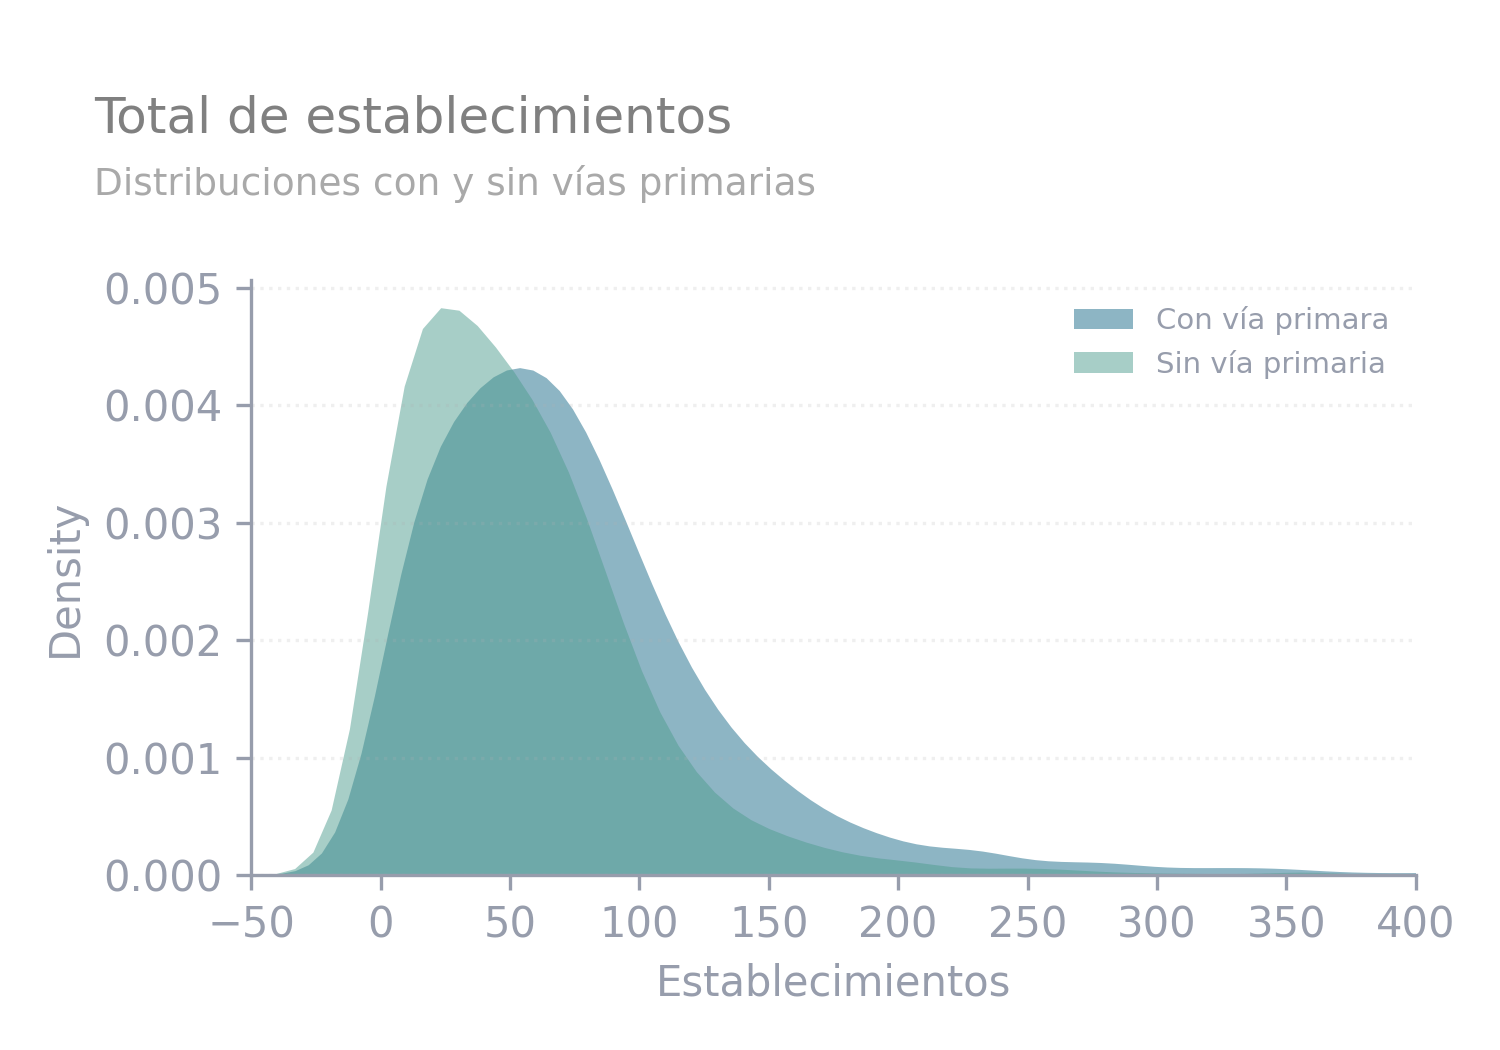
\includegraphics[width=.6\linewidth]{Imagenes/distribucion-establecimientos-cdmx-hexagonos.png}
\end{figure}

\begin{figure}
    \centering
    \caption{Establecimientos en la CDMX}
    \label{fig:establecimientos-mapa}
    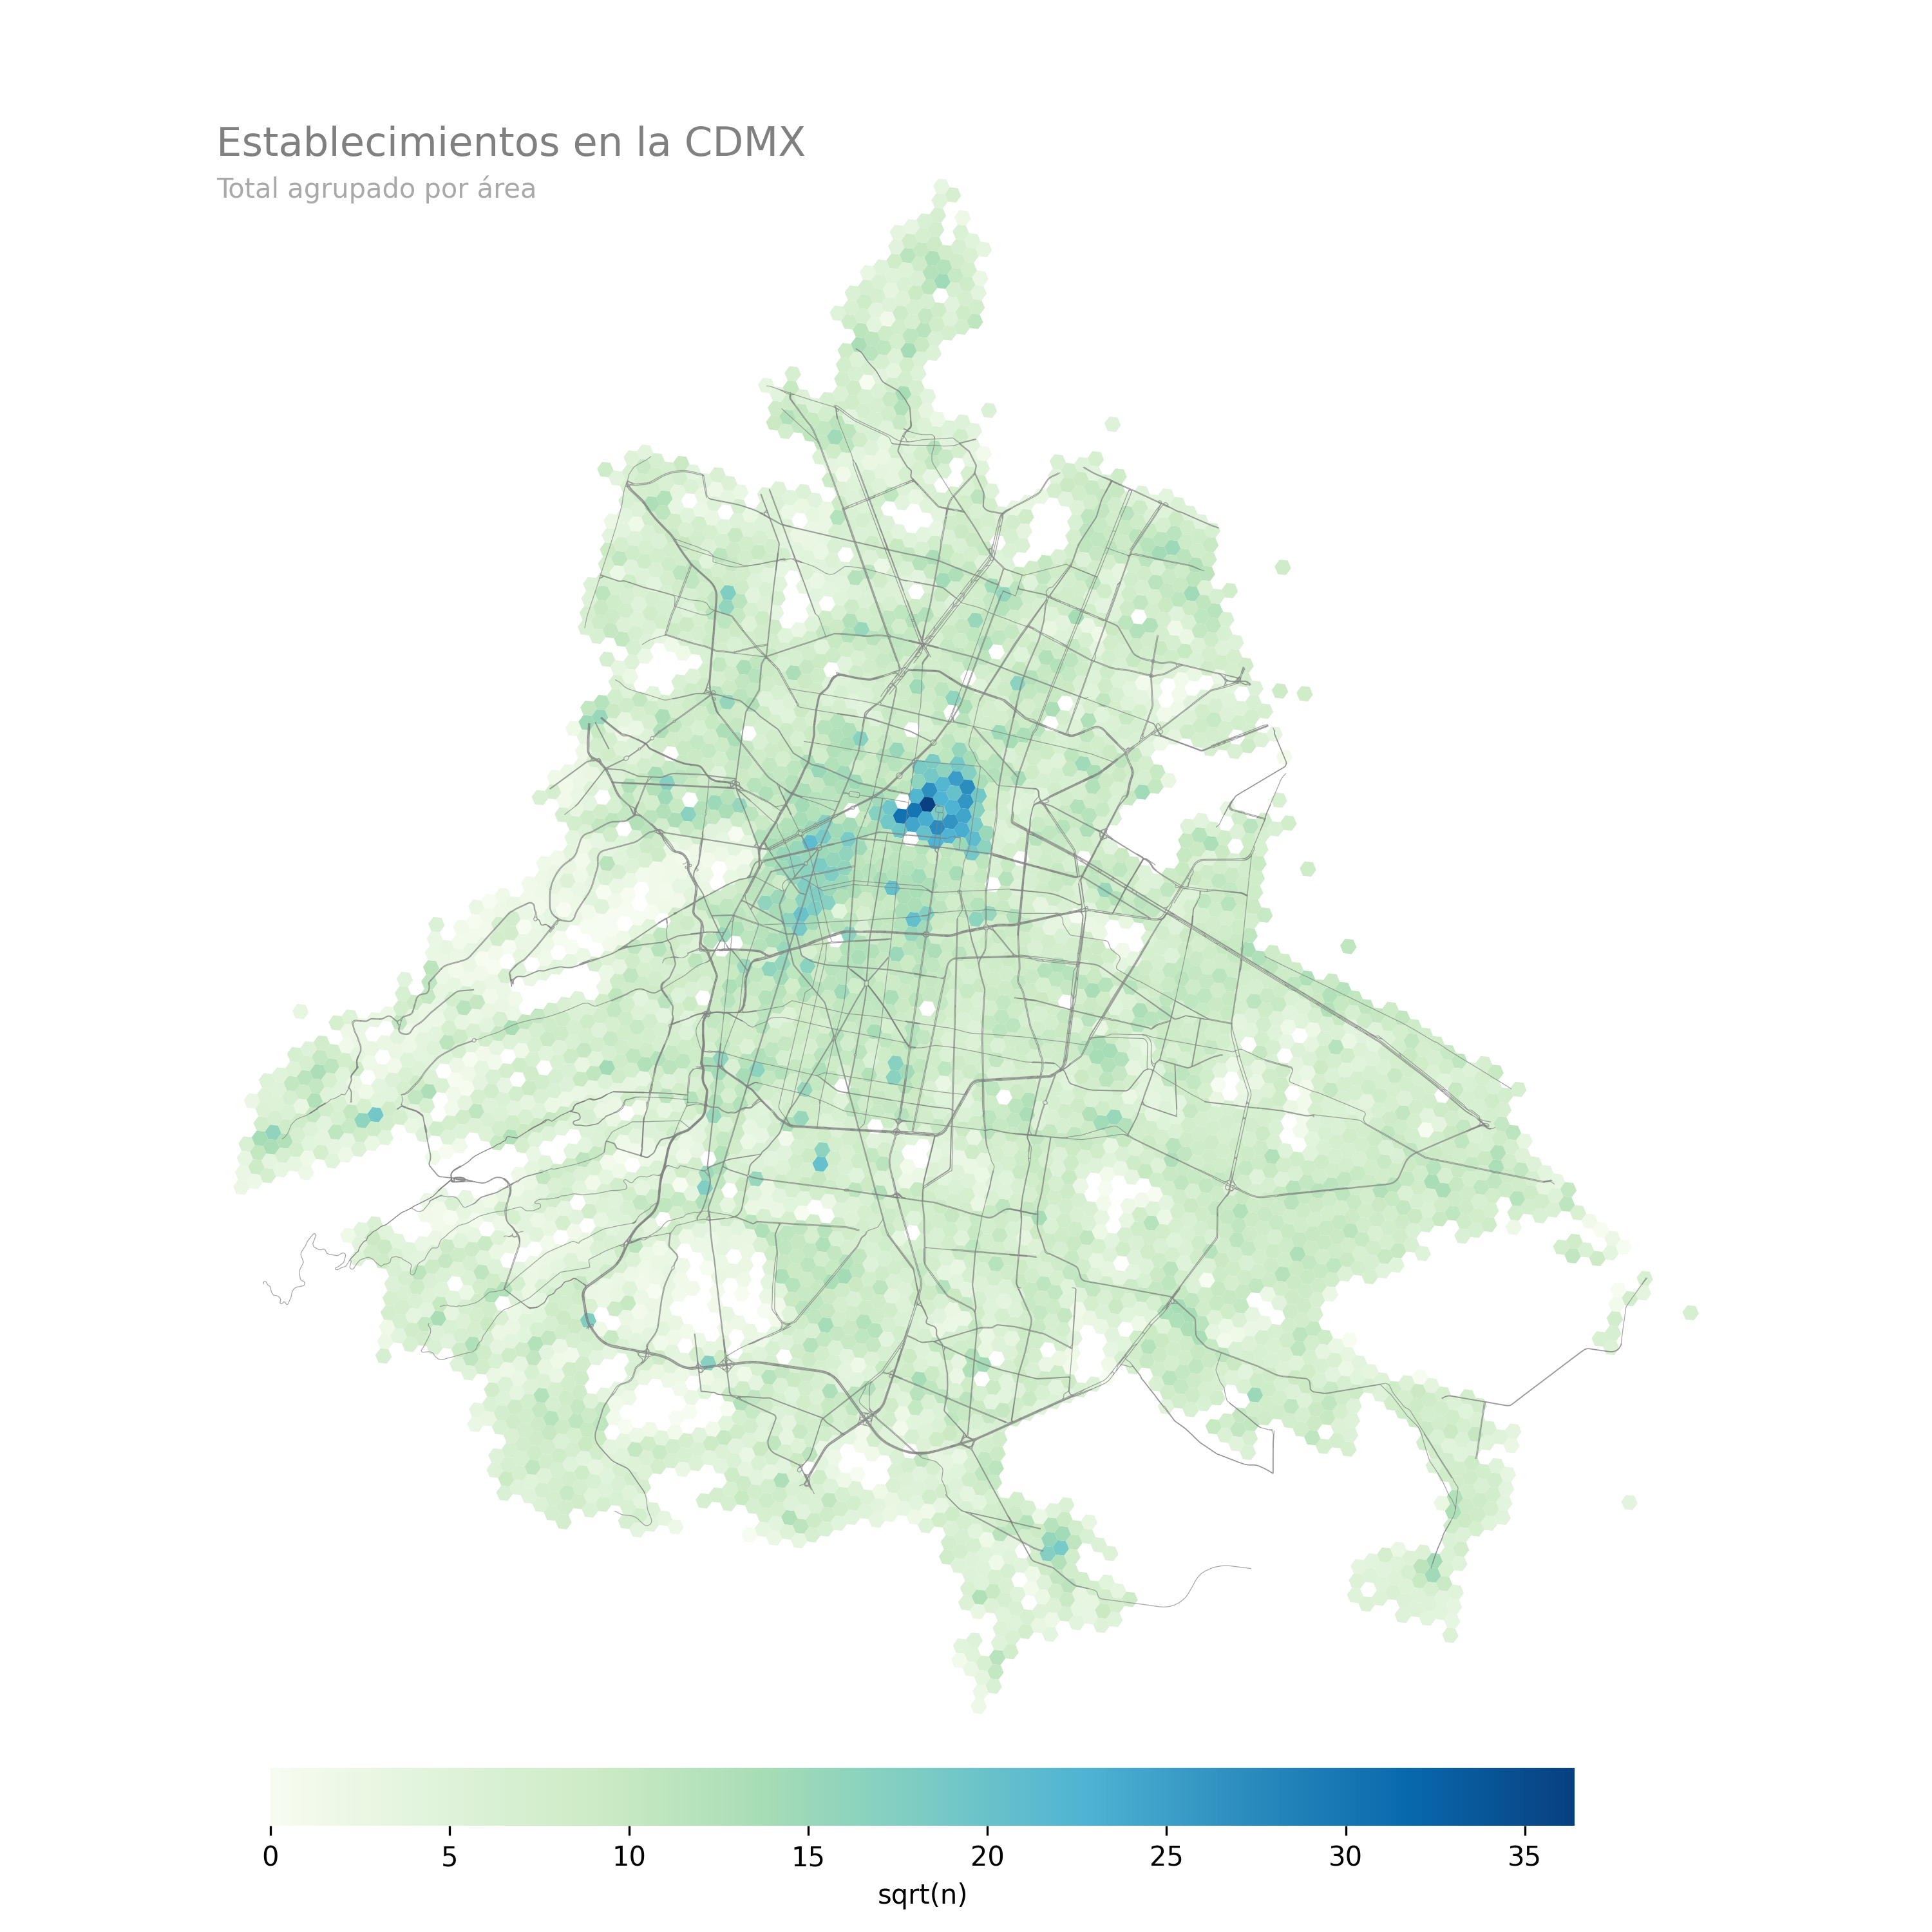
\includegraphics[width=1\linewidth]{Imagenes/establecimientos-en-la-cdmx.png}
\end{figure}
En conjunto, estas diferencias en velocidad reglamentaria, siniestros y nivel de actividad económica muestran que las zonas con y sin vías primarias corresponden a entornos viales y urbanos cualitativamente distintos. Una comparación directa entre ellas introduciría sesgos difíciles de manejar, incluso tras ajustar por covariables observables. Por este motivo, acoto el universo de análisis a áreas centradas sobre vías primarias y de acceso controlado. Con base en este universo más homogéneo, más adelante implemento un procedimiento de emparejamiento por \textit{propensity score}, que selecciona de entre los candidatos los controles más parecidos a cada unidad tratada y define la muestra final del análisis.

\section{Estrategia de identificación}

\subsection{Efecto de interés}
\noindent El objetivo de esta tesis es estimar el efecto causal de las cámaras de velocidad sobre la seguridad vial en su entorno inmediato. En particular, me interesa cuantificar cómo cambia el número mensual de incidentes viales en las áreas donde se ubican los radares, en comparación con lo que hubiera ocurrido en ausencia de cámaras. El efecto se estima por separado para el total de incidentes y para cada nivel de severidad, y para cada uno de los cinco radios.\\

En términos de inferencia causal, este efecto se interpreta como un \emph{average treatment effect on the treated} (ATT): el efecto promedio de contar con una cámara sobre las áreas efectivamente tratadas, tomando como contrafactual áreas de control emparejadas con características observables similares. Conviene precisar desde ahora sobre qué áreas tratadas se define este promedio. Como se explica más adelante, el análisis solo incluye a las áreas tratadas que encuentran un control comparable en los cinco radios, de modo que el ATT corresponde a ese subconjunto y no necesariamente a todas las cámaras del programa. En el capítulo 3 se describe cuántas áreas quedan fuera y en qué se distinguen de las demás.\\

\subsection{Alternativas de estimación}
\noindent Existen, en principio, varias formas alternativas de aproximarse a este problema. Una opción natural sería un ejercicio tipo \emph{before--after} en las áreas donde se instalaron las cámaras, comparando directamente el nivel de siniestros antes y después de abril de 2019. Sin embargo, esta aproximación es especialmente problemática en este contexto por dos razones. Primero, el periodo de estudio incluye el choque exógeno de la pandemia de COVID-19, que alteró de manera drástica los patrones de movilidad y, por tanto, la siniestralidad vial. Un simple \emph{before--after} confundiría los efectos de la pandemia con los del programa de fotocívicas. Segundo, incluso en ausencia de la pandemia, cualquier cambio en tendencias generales de accidentes en la ciudad podría ser erróneamente atribuido a las cámaras si no se cuenta con un grupo de comparación adecuado.\\

Otra alternativa sería estimar un modelo de diferencia en diferencias utilizando como controles todas las áreas elegibles que no recibieron cámaras. Sin embargo, como se discutió en la sección anterior, la asignación del programa no fue aleatoria: por diseño, las cámaras se instalaron en zonas con mayor riesgo vial. Usar de manera indiscriminada todas las demás áreas como contrafactual llevaría a comparar zonas sistemáticamente más peligrosas con otras estructuralmente distintas, y no hay razón para suponer que ambos grupos hubieran seguido trayectorias similares en ausencia del programa; es decir, el supuesto de tendencias paralelas resulta poco creíble.\\

Una tercera opción sería usar únicamente \emph{propensity score matching} (PSM): emparejar cada área tratada con un área de control parecida y comparar sus incidentes después del programa. El problema es que esa comparación mira un solo momento. Las cámaras empezaron a operar en una fecha concreta y se cuenta con información de las mismas áreas antes y después de esa fecha; perderíamos información muy valiosa si no consideráramos la naturaleza temporal de la intervención, por ejemplo, cualquier diferencia entre tratadas y controles que ya existiera antes del programa y que el emparejamiento no haya eliminado. Por ello, resulta más natural combinar el emparejamiento con un modelo de diferencia en diferencias.\\

En el capítulo 4 evalúo estas posibilidades con los mismos datos, para mostrar cuánto cambia la conclusión conforme se corrigen sus problemas, hasta llegar a la especificación principal.\\

\subsection{Emparejamiento}
\noindent La estrategia de esta tesis combina ambas herramientas: primero, utilizo el \emph{propensity score} para construir pares de áreas tratadas y de control que sean lo más comparables posible en términos de covariables observables; después, estimo sobre esta muestra emparejada un modelo de diferencia en diferencias con efectos fijos. De esta manera, el emparejamiento actúa como un paso previo que mejora la calidad del grupo de comparación, mientras que la estructura de panel permite aislar los cambios diferenciales en el tiempo asociados a la implementación del programa.\\

El \emph{propensity score} es la probabilidad de que un área cuente con una cámara de velocidad, condicional en sus covariables observables. Lo estimo con un modelo logístico cuyos regresores son características del área medidas antes del programa: su infraestructura vial, su siniestralidad en los tres años previos, incluida la tendencia de los incidentes, y la afluencia del Metro. El \emph{propensity score} resume así, en una sola dimensión, la información de las covariables relevantes para la asignación de las cámaras.\\

A partir del \emph{propensity score}, cada área tratada se empareja con el área de control más parecida, sin reemplazo, de modo que cada control se utiliza a lo más una vez. Esto garantiza que cada control represente un contrafactual similar a su área tratada, en lugar de reutilizar en exceso un pequeño conjunto de controles ``muy buenos'', lo que concentraría la inferencia en pocas zonas de la ciudad. Las áreas tratadas que no encuentran ningún control suficientemente parecido se excluyen, porque para ellas no existe una comparación defendible; este es el supuesto de soporte común. Como el emparejamiento se repite en cada radio, solo se conservan las áreas tratadas que encuentran pareja en los cinco, de modo que todos los radios estiman el efecto sobre las mismas unidades. El modelo logístico, el criterio de similitud y la evaluación del balance se detallan en el capítulo 3.\\

\subsection{Especificación}
\noindent Sobre la muestra emparejada estimo tres especificaciones de manera progresiva. La primera no incluye efectos fijos:
\begin{equation}
    Y_{it} = \alpha + \delta \, T_i + \lambda \, \text{Post}_t + \beta \, (T_i \times \text{Post}_t) + \varepsilon_{it}
    \label{eq:did1}
\end{equation}
donde $Y_{it}$ es el número de incidentes en el área $i$ durante el periodo $t$; $T_i$ indica si el área es tratada, y $\text{Post}_t$ indica si el periodo es posterior al 22 de abril de 2019. En ella, $\alpha$ es el promedio de los controles antes del programa, $\delta$ la diferencia entre tratadas y controles antes del programa, $\lambda$ el cambio de los controles después del programa y $\beta$, el coeficiente de interés, el cambio adicional que registraron las tratadas por encima del de sus controles.\\

La segunda introduce efectos fijos, tanto por área como por periodo, y se quitan los indicadores de tratamiento y de periodo posterior:
\begin{equation}
    Y_{it} = \alpha_i + \lambda_t + \beta \, (T_i \times \text{Post}_t) + \varepsilon_{it}
    \label{eq:did2}
\end{equation}
donde $\alpha_i$ son efectos fijos por área, que capturan las características de cada área que no cambian en el tiempo, y $\lambda_t$ son efectos fijos por periodo, que capturan lo que le ocurre a todas las áreas en un mismo periodo. Como el panel está balanceado y todas las cámaras entraron en vigor el mismo día, $\beta$ es idéntico en las ecuaciones~\eqref{eq:did1} y~\eqref{eq:did2}.\\

La tercera, que es la especificación principal, agrega covariables interactuadas con el periodo posterior:
\begin{equation}
    Y_{it} = \alpha_i + \lambda_t + \beta \, (T_i \times \text{Post}_t) + \sum_{k=1}^{8} \gamma_k \, (X_{ik} \times \text{Post}_t) + \varepsilon_{it}
    \label{eq:did}
\end{equation}
donde $X_{ik}$ son ocho características de cada área. En las tres especificaciones el modelo es lineal y se estima por mínimos cuadrados ordinarios, de modo que $\beta$ se interpreta directamente en incidentes por mes; para facilitar su lectura, se reporta también como porcentaje del promedio mensual de incidentes del grupo de control antes del programa.\\

Las covariables se agregan porque el emparejamiento no deja un balance perfecto: después de emparejar persisten diferencias pequeñas en algunas covariables, y si esas características influyen en cómo evolucionan los incidentes después de 2019, podrían confundirse con el efecto de las cámaras. Estas covariables describen cada área antes del programa: las de infraestructura vial salen de la red vial, y la de afluencia del Metro es el promedio de los tres años previos. Cada una tiene un solo valor por área, que no se actualiza después de abril de 2019. Esto es deliberado: si las cámaras modificaron, por ejemplo, el tránsito o la afluencia del Metro a su alrededor, usar los valores posteriores al programa como control absorbería parte del efecto que se busca medir. Al ser fijas en el tiempo, por sí solas las absorben los efectos fijos de área; lo que aporta información es su interacción con $\text{Post}_t$, que permite que áreas con distinta infraestructura vial o distinta afluencia del Metro tengan cambios distintos después del programa sin atribuírselos a la cámara.\\

Por eso entran las siete covariables de infraestructura vial y la de afluencia del Metro, pero no las de siniestralidad previa: interactuar el nivel previo de incidentes con el periodo posterior equivaldría a suponer que ese nivel determina la evolución posterior, que es justamente lo que el supuesto de tendencias paralelas establece que no ocurre. Las covariables de siniestralidad se balancean en el emparejamiento, pero no entran al modelo.\\

Los efectos fijos por periodo no son un control de la pandemia. Capturan lo que le ocurre a todas las áreas en un mismo periodo, de modo que la parte del choque que fue común a tratadas y controles queda fuera de $\beta$, como se discutió en la sección~\ref{sec:ventana}. La parte que pudo afectar de forma distinta a ambos grupos no la quita ningún efecto fijo; se evalúa con el efecto por año que se describe más adelante.\\

\subsection{Inferencia}
\noindent Los errores estándar se agrupan por componente traslapada. Algunas áreas tratadas se traslapan parcialmente sin llegar a fusionarse, y registran algunos de los mismos incidentes, por lo que no son observaciones independientes. Cada grupo de áreas tratadas conectadas por algún traslape forma un \emph{cluster}; los controles, que no se traslapan con ninguna otra área, forman cada uno el suyo.\\

Estos errores estándar, sin embargo, tratan los pares emparejados como si fueran fijos, cuando en realidad se construyeron con los mismos datos: con otra muestra, el \emph{propensity score} sería distinto y el emparejamiento elegiría otros controles. Para incorporar esa incertidumbre, calculo los intervalos de confianza con un \emph{bootstrap} que repite el proceso completo. En cada una de 2,000 repeticiones se remuestrean, con reemplazo, las áreas tratadas y el conjunto de controles candidatos, de modo que las áreas de un mismo \emph{cluster} entran o salen juntas; sobre esa muestra se vuelve a estimar el modelo logístico, se rehace el emparejamiento con las mismas reglas y se estima de nuevo el modelo de diferencia en diferencias. El intervalo de confianza al 95\% se construye con los percentiles 2.5 y 97.5 de los coeficientes obtenidos. Las limitaciones de este procedimiento se discuten en las conclusiones.\\

\subsection{Evaluación de los supuestos}
\noindent El supuesto de tendencias paralelas no puede probarse directamente, porque se refiere a lo que hubiera ocurrido sin el programa. Lo que sí puede revisarse es si tratadas y controles ya se separaban antes de 2019. Para ello hago un \emph{event study}: la misma especificación~\eqref{eq:did}, pero con un coeficiente de tratamiento para cada año de la ventana, anterior o posterior al programa, y con el año inmediatamente anterior a las fotocívicas como referencia. Las covariables también se interactúan con cada año. Si las tendencias eran paralelas, los coeficientes de los años previos deberían ser cercanos a cero; además de revisarlos uno por uno, se prueba conjuntamente que todos sean cero.\\

Como ya se adelantaba, verifico también que la pandemia no esté cargando los resultados. Para esto, estimo una variante en la que el indicador $\text{Post}_t$ se separa en tres indicadores anuales, cada uno del 22 de abril al 21 de abril del año siguiente: el primero cierra con el primer mes del confinamiento, el segundo corresponde al año de la pandemia y el tercero va de 2021 a 2022. Si el efecto estimado se debiera a un choque de la pandemia que afectó de forma distinta a tratadas y controles, el coeficiente del segundo año debería apartarse de los demás. Los resultados de ambas pruebas se presentan en el capítulo 4.\\
